\documentclass{article}

% if you need to pass options to natbib, use, e.g.:
% \PassOptionsToPackage{numbers, compress}{natbib}
% before loading nips_2017
%
% to avoid loading the natbib package, add option nonatbib:
% \usepackage[nonatbib]{nips_2017}

\usepackage[final,nonatbib]{nips_2017}

% to compile a camera-ready version, add the [final] option, e.g.:
% \usepackage[final]{nips_2017}

\usepackage[utf8]{inputenc} % allow utf-8 input
\usepackage[T1]{fontenc}    % use 8-bit T1 fonts
\usepackage{hyperref}       % hyperlinks
\usepackage{url}            % simple URL typesetting
\usepackage{booktabs}       % professional-quality tables
\usepackage{amsfonts}       % blackboard math symbols
\usepackage{nicefrac}       % compact symbols for 1/2, etc.
\usepackage{microtype}      % microtypography
\usepackage{graphicx}
\usepackage{amsmath}
\usepackage{wrapfig}
\usepackage{subcaption}
\usepackage[numbers]{natbib}
\usepackage[toc,page]{appendix}
\bibliographystyle{plainnat}

\title{An Error Detection and Correction Framework for Connectomics}
\author{
	Jonathan Zung\\
	Princeton University\\
	jzung@princeton.edu
	\And
	Ignacio Tartavull\\
	Princeton University\\
	tartavull@princeton.edu
	\And
	H. Sebastian Seung\\
	Princeton University\\
	sseung@princeton.edu
	\And
}
\begin{document}

\maketitle

\begin{abstract}
We define and study error detection and correction tasks that are
useful for 3D reconstruction of neurons from electron microscopic
imagery, and for instance segmentation more generally.  The error
detection task takes as input the original image and a binary mask
representing a candidate object. The desired output is a map of split
and merge errors in the object. The error correction task is
formulated as object mask reduction. The input is the original image
and a candidate object mask. The task is to reduce the object mask to
generate the true object. We train multiscale 3D convolutional
networks to perform both tasks, and then show how the nets can be
combined to achieve significant improvements in segmentation
accuracy. Namely, the error detecting net is used to create the
object mask that is the input to the error correcting net.
\end{abstract}

\section{Introduction}
While neuronal circuits can be reconstructed from volumetric electron
microscopic imagery, the process has historically
\cite{white1986structure} and even recently \cite{schmidt2017axonal}
been highly laborious. One of the most time-consuming reconstruction
tasks is the tracing of the brain's ``wires,'' or neuronal branches.
This task is an example of instance segmentation, and can be automated through computer detection of the boundaries between neurons. Convolutional nets were first applied to neuronal boundary detection a decade ago \cite{boundary_detection, jain2007supervised}.
Since then convolutional nets have become the standard approach, and
the accuracy of boundary detection has become impressively high  \cite{li2017deep, beier2017multicut, kisuk, funke2017deep}.

Given the low error rates, it becomes helpful to think of subsequent processing steps in terms of modules that detect and correct errors. In the error detection task (Fig. 1A), the input is the original image and a binary mask that represents a candidate object. The desired output is a map containing the locations of split and merge errors in the candidate object. Related work on this problem has been restricted to detection of merge errors only by either hand-designed \cite{multipass} or learned \cite{mergenet} computations.

In the error correction task (Fig. 1B), the input is again the original image and a binary mask that represents a candidate object. The candidate object mask is assumed to be a superset of a true object, which is the desired output. With this assumption, error correction is formulated as \emph{object mask reduction}.
Object mask reduction can be regarded as the splitting of undersegmented objects to create true objects. In this sense, it is the opposite of agglomeration, which merges oversegmented objects to create true objects \cite{lash,gala}. Object mask reduction can also be viewed as the \emph{subtraction} of voxels from an object to create a true object. In this sense, it is the opposite of a flood-filling net \cite{floodfilling,januszewski2017high}, each iteration of which is the \emph{addition} of voxels to an object to create a true object. Flood-filling nets are closely related to other work on instance segmentation in connectomics \cite{multipass} and computer vision \cite{recurrent_instance_seg_1, recurrent_instance_seg_2}.  The task of generating an object mask de novo from an image has also been studied in computer vision [citation from Kisuk].

We implement both error detection and error correction using 3D multiscale convolutional networks.  One can imagine multiple uses for these nets in a connectomics pipeline. For example, the error-detecting net could be used to reduce the amount of labor required for proofreading by directing human attention to locations in the image where errors are likely. This labor reduction could be substantial because the declining error rate of automated segmentation has made it more time-consuming for a human to find an error.

We find it especially interesting and natural to combine the error-detecting and error-correcting nets in the following way. To create the candidate object mask for the error-correcting net from a baseline segmentation, one can simply take the union of all erroneous segments as found by the error-detecting net. Since the typical error rate in the baseline segmentation is already low, there is often not much for the error-correcting net to erase and the task is relatively easy.

%Furthermore, we observe the interesting phenomenon that it is often much easier to detect an error than to find the correct segmentation. Indeed, humans are usually able to detect a segmentation error without even looking at the original image; they look for neurites that terminate prematurely or x-shaped junctions indicating incorrectly merged segments. However, the incredible density of information in neural tissue makes searching for the correction difficult.

%Our approach is to decompose the problem of refining a given segmentation into two easier problems: error detection and error correction. As a wise man once said, recognizing your faults is the first step towards fixing them. We hypothesize that thanks to the distinctive shapes of neurons, recognizing an error is much easier than finding the correct answer. 

%Conversely, an error detection module makes error correction much easier. Once we remove from consideration all objects which do not contain an error, the visual crowding problem is alleviated. Choosing the correct extension of a neurite is easy when there are only a few choices available. Furthermore, we can afford to apply a relatively expensive error correction procedure as it does not need to be applied everywhere.

%In this paper, we will demonstrate the feasibility of high quality error detection. We will also demonstrate the effectiveness of error detection in directing the attention of an error correction module. We expect our error detector will be independently useful for directing human proofreading effort.

%We also argue that the error detection task is better posed than the supervoxel agglomeration task. Given two objects which already contain errors, it is often unclear whether the segmentation improves after they have been merged. In \cite{lash}, the authors resolve this ambiguity by training to predict the change in rand score from a proposed merge.

%While $\cite{floodfilling}$ performs inference densely, we selectively apply our error correction module near likely errors. This comparatively reduces our computational cost. We sacrifice end-to-end training for this advantage.

%Our main novelty relative to their approach is the use of the advice of an error detector to bias flood filling. While they present their network with a partially reconstructed object and ask for a completion, we present our network with the union of all possibly incorrect segments in a window and ask the network to split out a single object. Since the typical error rate is already low, this ``advice'' on which objects to consider is informative and significantly improves the performance of our flood filling networks. 

\section{Error Detection}
\subsection{Task Specification}
\begin{figure}
\begin{center}
	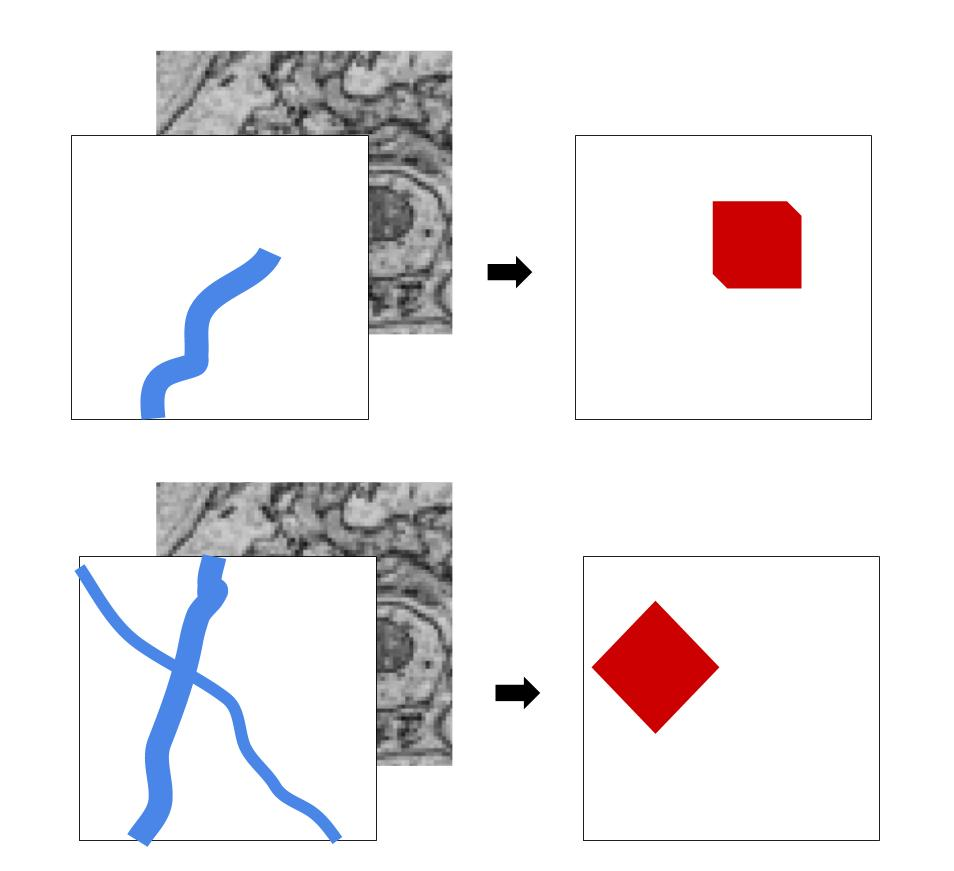
\includegraphics[width=0.65\linewidth]{detection_task.jpg}
	\caption{Input to the error detector on the left and the corresponding error map on the right.}
	\label{fig:error_detection_cartoon}
\end{center}
\end{figure}
Given a single segment in a proposed segmentation presented as a binary image $Obj$, the error detection task is to produce a second binary image called the \textit{error map}, denoted $Err_{p_x\times p_y \times p_z}(Obj)$. The definition of the error map depends on a choice of a window size $p_x \times p_y \times p_z$. A pixel $i$ in the error map is 1 iff the restriction of the input image to a window centred at $i$ of size $p_x \times p_y \times p_z$ is pixel-wise equal to the restriction of some object in the ground truth. Observe that the error map is sensitive to both split and merge errors.

A smaller window size allows us to localize errors more precisely. On the other hand, if the window radius is less than the width of a typical boundary, it is possible that two objects participating in a merge error never appear in the same window. These merge errors would not be classified as an error in any window. 

We could use a less stringent measure than pixel-wise equality that disregards small perturbations of the boundaries of objects. However, our proposed segmentations are all composed of the same building blocks (supervoxels) as the ground truth segmentation, so this is not an issue for us.

We define the \textit{combined error map} as $\sum_{Obj} Err(Obj) * Obj$ where $*$ represents pointwise multiplication. In other words, we restrict the error map for each object to the object itself, and then sum the results. The figures in this paper show the \textit{combined error map}.

\subsection{Architecture}
We take a fully supervised approach to error detection. We implement error detection using a multiscale 3D convolutional neural network. The architecture is detailed in ~\ref{appendix:architecture}. Its design is informed by experience with convolutional networks for boundary detection (see \cite{kisuk}) and reflects recent trends in neural network design \cite{unet,resnet}. Its field of view is $P_x\times P_y\times P_z=318\times 318\times 33$ (which is roughly cubic in physical size given the anisotropic resolution of our dataset). The network computes (downsamplings of) $Err_{46 \times 46 \times 7}$, $Err_{98 \times 98 \times 12}$, and $Err_{318 \times 318 \times 33}$. At test time, we perform inference in overlapping windowsand conservatively blend the output from overlapping windows using a maximum operation.

We trained two variants, one of which takes as input only $Obj$, and another which additionally receives as input the original image. 

\section{Error Correction}
\subsection{Task Specification}
\begin{figure}
\begin{center}
	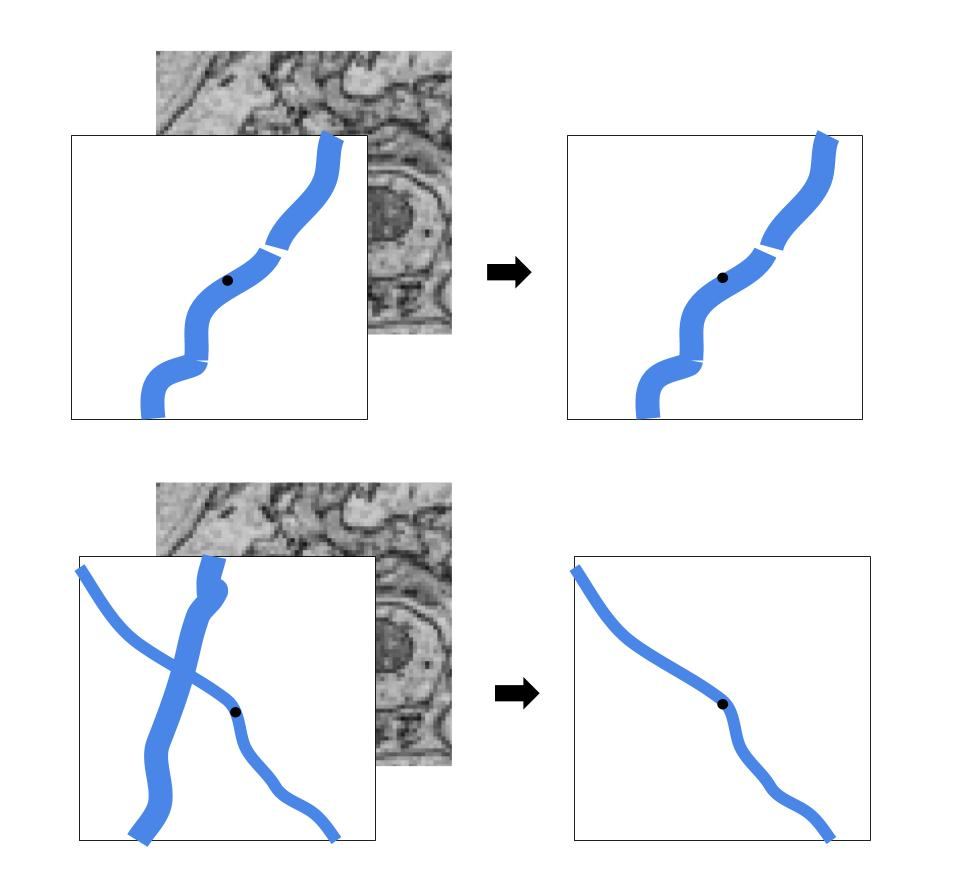
\includegraphics[width=0.65\linewidth]{correction_task.jpg}
	\caption{Desired input and output for the erasure network. In the first case there is nothing to erase, while in the second case the object not overlapping the central pixel is erased.}
	\label{fig:error_correction_cartoon}
\end{center}
\end{figure}
The error correction module has two inputs: first, an image patch of size $P_x\times P_y\times P_z$ and second a binary image encoding the union of several objects. The error correction task is to erase all objects except for the object overlapping the central pixel.

At test time, the input binary image will be the union of all objects with a detected error.

\subsection{Architecture}
Yet again, we implement error correction using a multiscale 3D convolutional neural network. The architecture is detailed in ~\ref{appendix:architecture}. One difficulty with training a neural network to reconstruct the object containing the central pixel is that the desired output can change drastically as the central pixel moves between objects. We use an intermediate representation whose role is to soften this dependence on the location of the central pixel. The desired intermediate representation is a $k$ dimensional vector $v(x,y,z)$ at each point $(x,y,z)$ such that points within the same object have similar vectors and points in different objects have different vectors. We transform this vector field into a binary image $M$ representing the object overlapping the central pixel as follows:

\begin{equation*}
	M(x,y,z)=\exp(-||v(x,y,z)-v(P_x/2,P_y/2,P_z/2)||^2)
\end{equation*}

When an over-segmentation is available, we replace $v(P_x/2,P_y/2,P_z/2)$ with the average of $v$ over the supervoxel containing the central pixel. Note that we backpropagate through the transform $M$, so the vector representation may be seen as an implementation detail and the output of the network is just a binary image.


\section{Putting it Together}

\begin{figure}
\begin{center}
	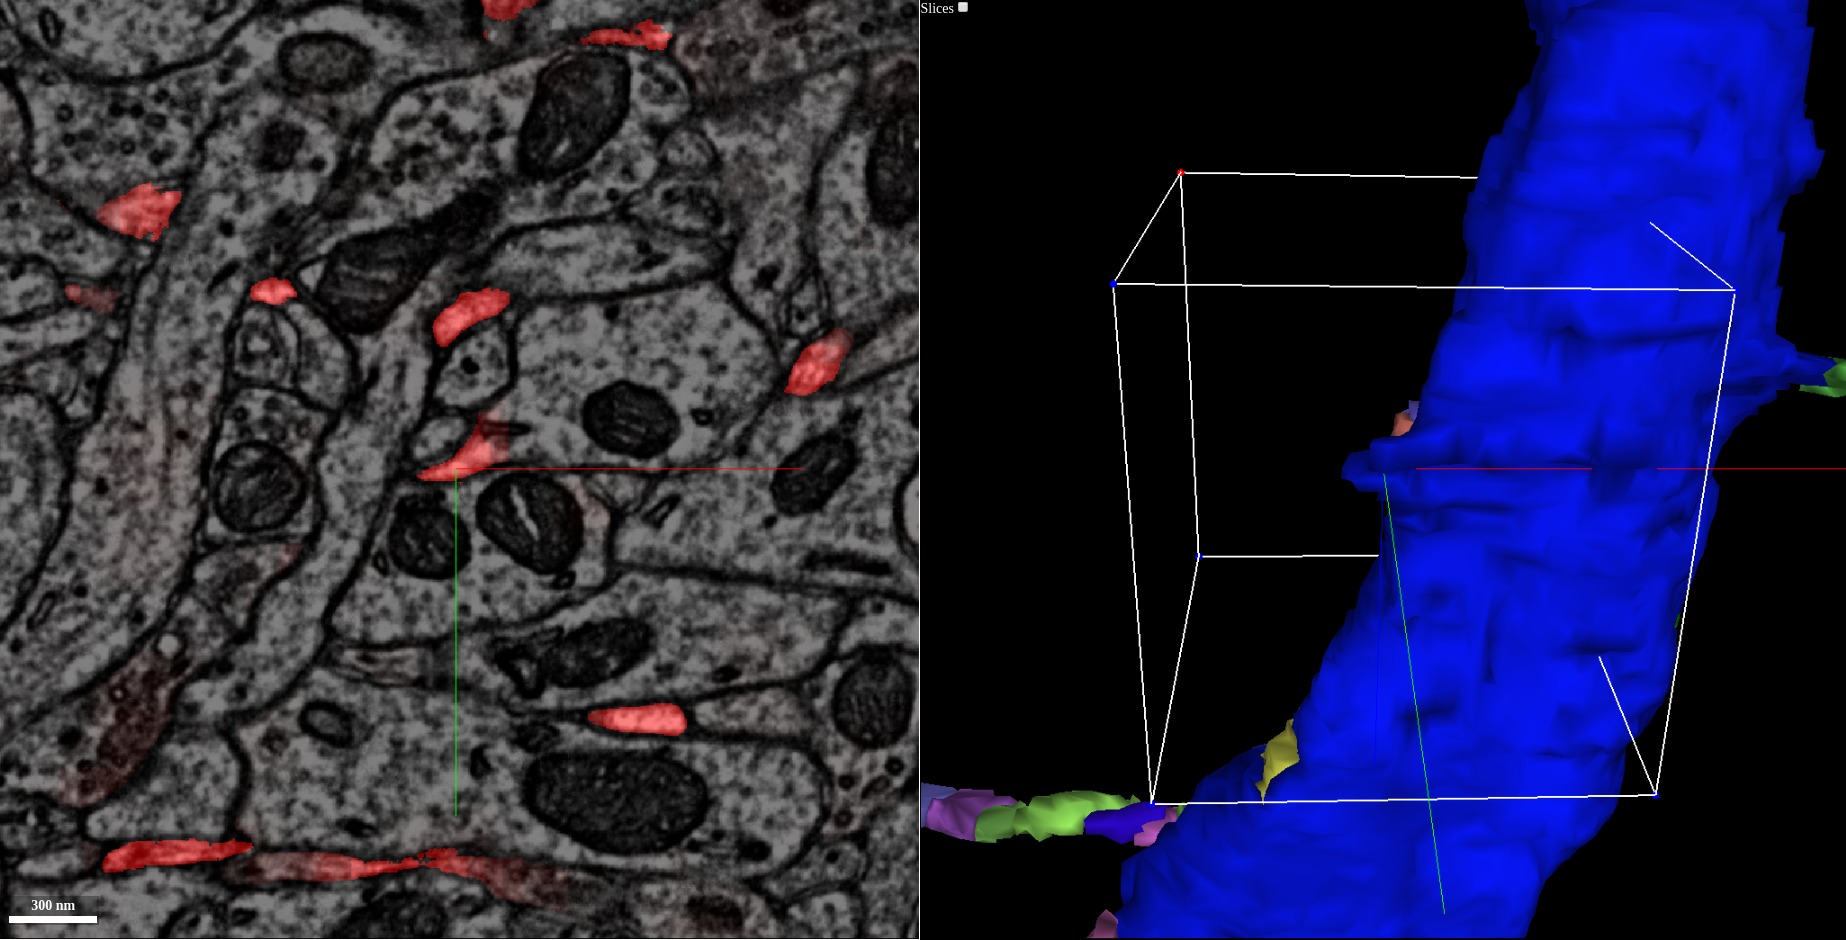
\includegraphics[width=0.65\linewidth]{errors.jpg}
	\caption{An example of a mistake in the initial segmentation. The dendrite is missing a spine. The red overlay on the left shows the combined error map; the stump in the centre of the image was clearly marked as an error.}

	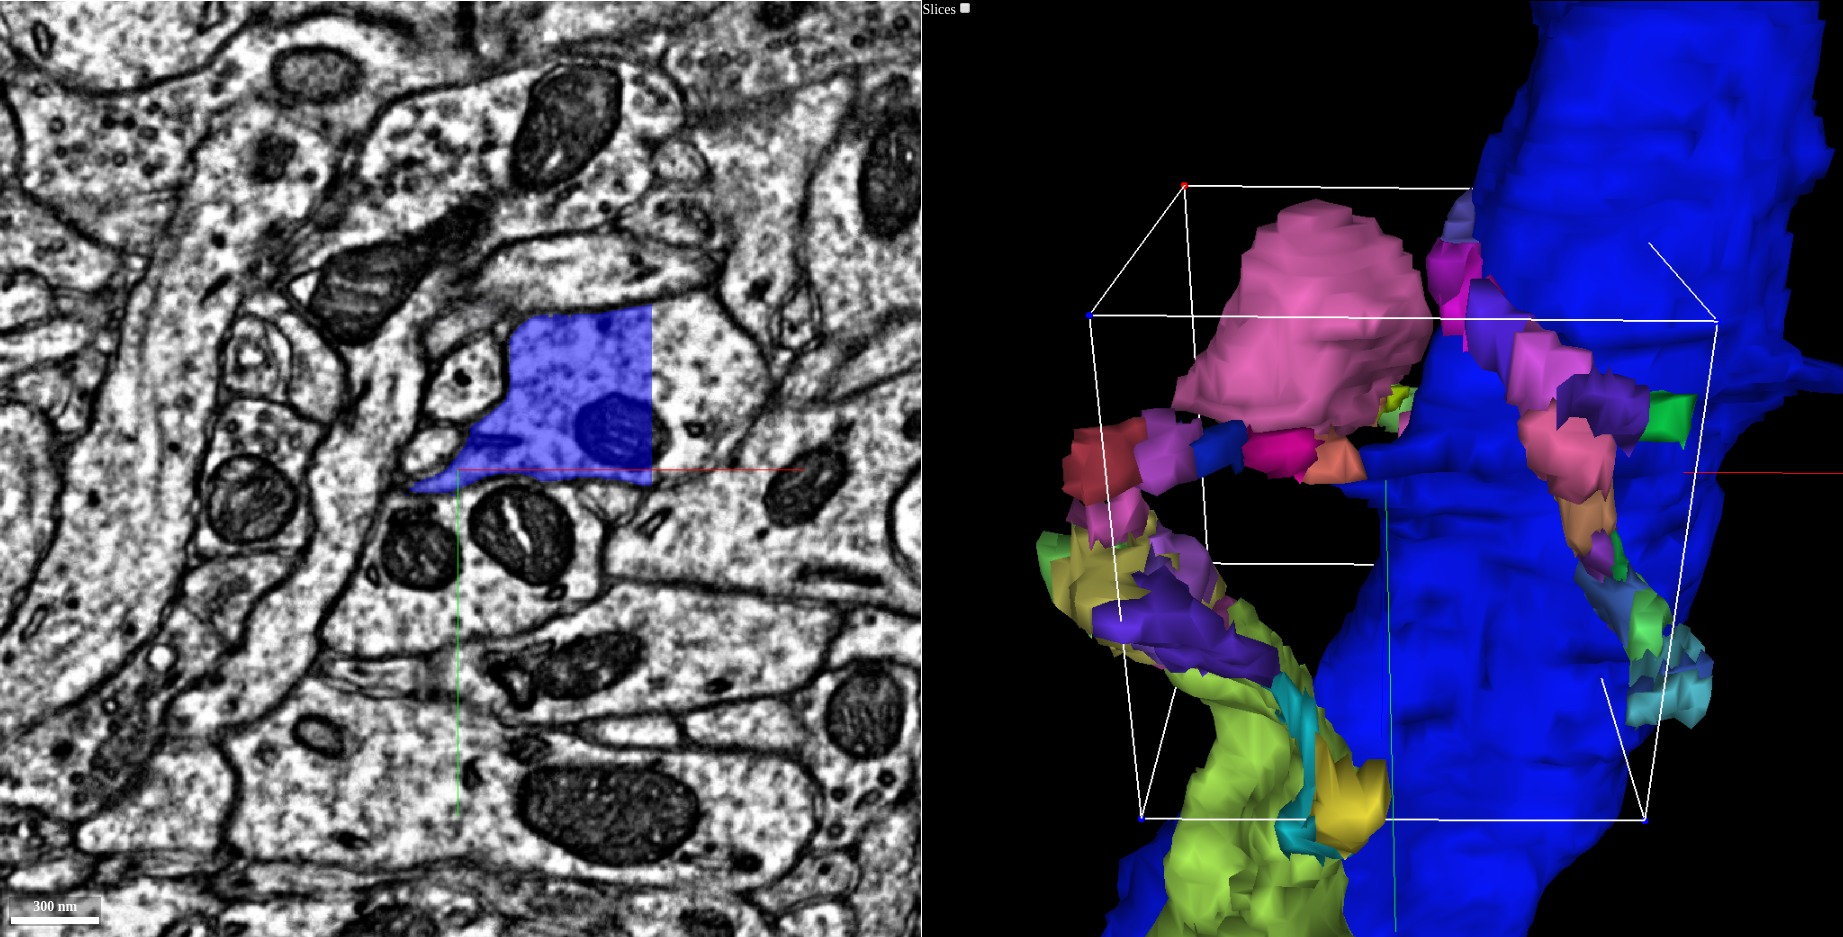
\includegraphics[width=0.65\linewidth]{neighbours.jpg}
	\caption{The right shows all objects which contained  a detected error in the vicinity. This is the ``advice'' image which is provided as an auxiliary input to the flood filling network. For clarity, these objects were clipped to lie within the white box representing the field of view of our flood filling network. The output of the floodfilling network is overlaid in blue on the left.}

	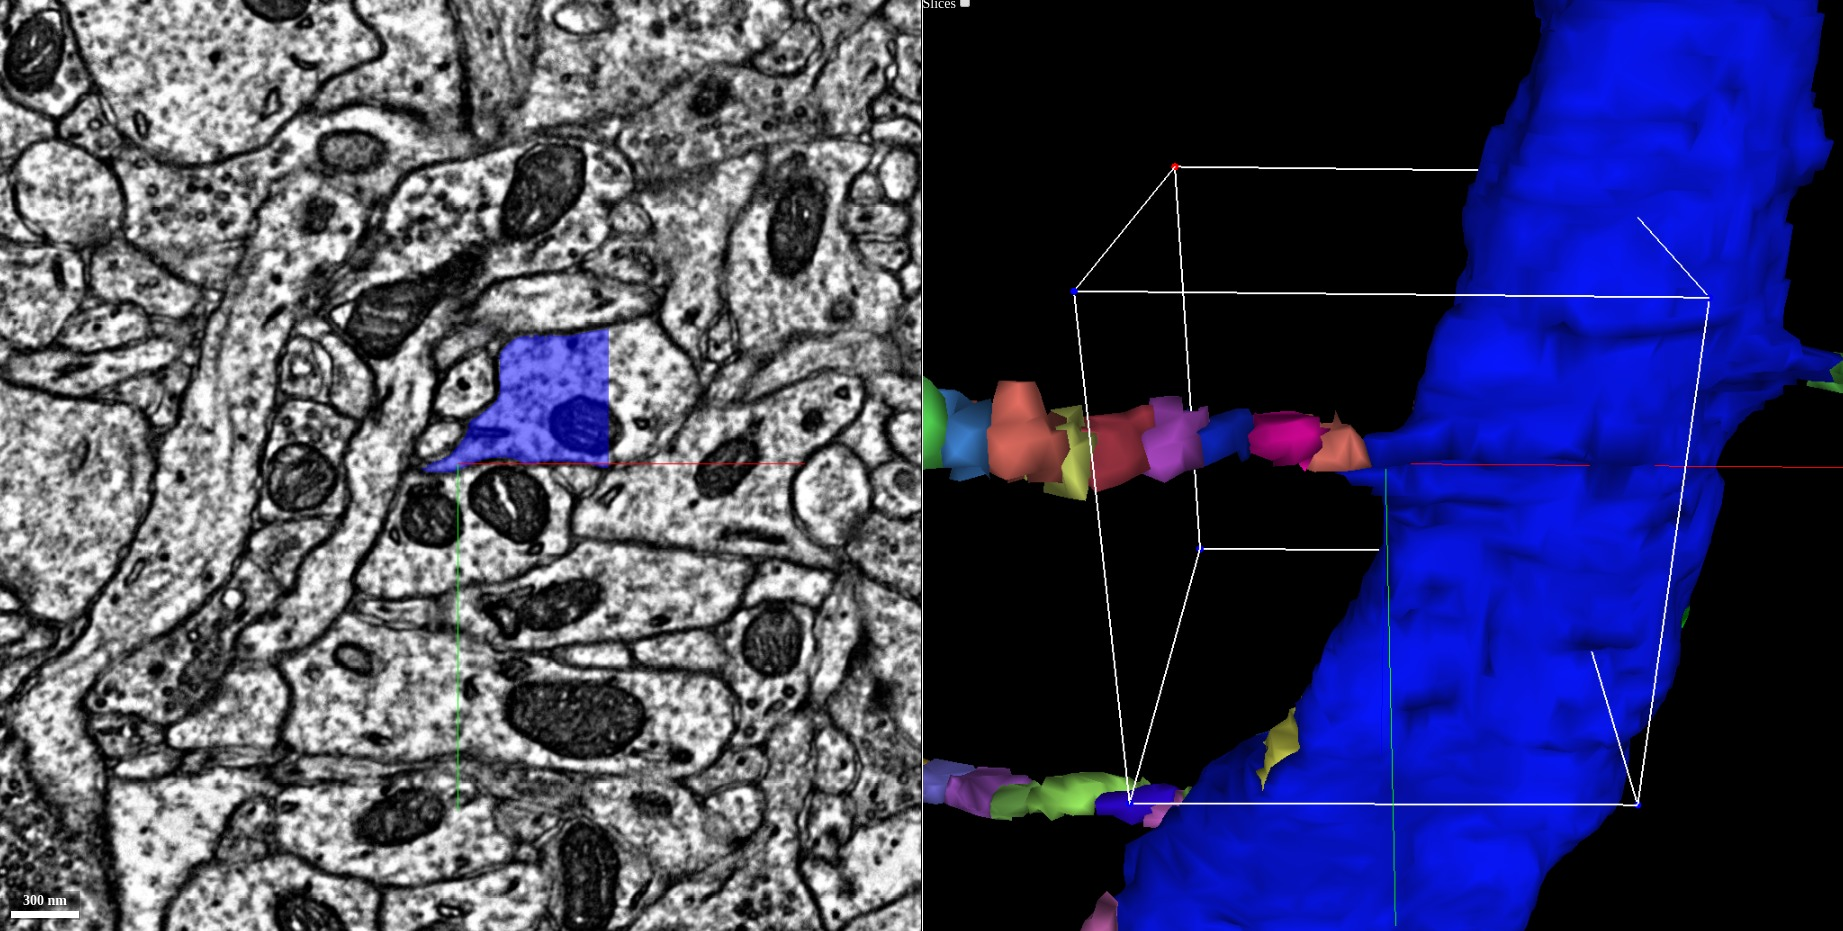
\includegraphics[width=0.65\linewidth]{final.jpg}
	\caption{The supervoxels assembled in accordance with the output of the flood filling network.}
\end{center}
\end{figure}
In this section, we describe how our error detectors and error correctors are combined at test time. We begin with a proposed segmentation whose remaining errors are assumed to be sparsely distributed. During the error correction phase, we iteratively update a segmentation represented as a graph $G$ whose vertices are segments in a strict over-segmentation (henceforth called supervoxels) and whose connected components are segments in the proposed segmentation. We also maintain the combined error map associated with the current segmentation. We binarize the error map by thresholding at 0.25.

Now we iteratively choose a location $l=(x,y,z)$ which has value 1 in the combined error map. In a $P_x \times P_y \times P_z$ window centred on $l$, we prepare an input for the error corrector by taking the union of all segments containing at least one white pixel in the error map. We apply the error correction network to produce a binary image $M$ representing the object containing the central pixel. For each supervoxel $S$, let $M(S)$ denote the average value of $M$ inside $S$. If $M(S) \not \in [0.1,0.9]$ for all $S$ in the relevant window, add to $G$ a clique on $\{S | M(S) > 0.9\}$ and delete from $G$ all edges between $\{S | M(S) < 0.9\}$ and $\{S | M(S) > 0.9\}$. The effect of this is to update $G$ to locally agree with $M$. Finally, we update the combined error map by applying the error detector at all locations where its decision could have changed.

We would like to iterate until every location is zero in the error map or has been covered by a window at least twice by the error corrector. This stopping criterion guarantees that the algorithm terminates.

%In this section, we present a greedy algorithm which combines the error detector and the error corrector to greedily update an initial segmentation. We assume that we are provided with an initial segmentation along with a strict over-segmentation. We term the segments in the over-segmentation supervoxels. Throughout the error correction phase, we maintain a graph whose vertices are supervoxels and whose connected components are segments in the proposed segmentation.

%Let $L$ be a list of locations densely sampled from the image. We say that an error is detected at a location of the the error detector reports a value of >0.25 on a window centred at that location. For each location in the 

\section{Experiments}
\subsection{Dataset}

%Our dataset was culled from an unfortunate soul named Pinky. He had a big heart but a small brain, which made him perfect for our experiment. May he rest in peace.

Our dataset is a sample of mouse visual cortex acquired using transmission electron microscopy at the Allen Institute for Brain Science. The voxel resolution is $3.6\text{nm} \times 3.6\text{nm} \times 40\text{nm}$.

A team of tracers produced a gold standard dense reconstruction of $850$ Mvoxels. This volume was used to train the boundary detection networks. We applied the resulting boundary detector to a larger volume of size $5700$ Mvoxels.  Tracers corrected the resulting segmentation. This bootstrapped ground truth was used to train the error detector and error corrector. A subvolume of size $910$ Mvoxels was reserved for validation, and two volumes of size $910$ Mvoxels were reserved for testing.

Producing the gold standard segmentation required a total of $\sim900$ tracer hours, while producing the bootstrapped ground truth required $\sim 670$ tracer hours.

\subsection{Baseline Segmentation}
Our baseline segmentation was produced using a standard pipeline of multiscale convolutional neural networks for boundary detection, watershed, and mean affinity agglomeration. A similar pipeline is described in detail in  \cite{kisuk}. The segmentation performance values reported for the baseline are taken at a mean affinity agglomeration threshold of 0.23, which minimizes the total variation of information error metric on the test volume.

\subsection{Sampling Procedure}
\label{sec:sampling}
In this section, we describe our procedure for choosing a random point location in a segmentation. Uniformly random sampling is unsatisfactory since large objects such as dendritic trunks will be overrepresented. Instead, given a segmentation, we sample a location $x,y,z$ with probability inversely proportional to the fraction of a window of size $128\times 128 \times 16$ centred at $x,y,z$ which is occupied by the object containing pixel $x,y,z$.

\subsection{Error Detection Training Data}
An initial segmentation containing errors was produced using our baseline boundary detection network combined with mean affinity agglomeration at a threshold of 0.3. Point locations were sampled according to the sampling procedure specified in \ref{sec:sampling}. We augmented all of our data with rotations and reflections. 

\subsection{Error Correction Training Data}
We sampled locations in the ground truth segmentation as in $\ref{sec:sampling}$. At each location $x,y,z$, we generated a training example as follows. We selected a random subset of the objects in the window centred on $x,y,z$ including the object overlapping the central pixel. (To be precise, we chose a number $p$ uniformly at random from $[0,1]$, and then selected each segment in the window with probability $p$ in addition to the central object.) The input is a binary image representing the union of the selected objects along with the original EM image, and the desired output is a binary image representing only the central object. The dataset was augmented with rotations, reflections, simulated misalignments and missing sections.

Note that this training procedure is completely independent of the error detector and the baseline segmentataion.


\subsection{Error Detection Results}
To measure the quality of error detection, we densely sampled points in our test volume. In order to remove ambiguity over the precise location of errors, we sampled only points which contained an error within a surrounding window of size $40\times 40 \times 4$ or did not contain an error within a surronding window of size $80 \times 80 \times 8$. Precision and recall simultaneously exceed 90\% (see figure \ref{fig:error_detection_pr}). Empirically, many of the false positive examples come where a dendritic spine head curls back and touches its trunk. These examples locally appear to be incorrectly merged objects.

We trained one error detector with access to the original image and one without. The network's admirable performance even without access to the image as seen in figure ~$\ref{fig:error_detection_pr}$ supports our hypothesis that error detection is a relatively easy task and can be performed using only shape cues.
\begin{figure}
\begin{center}
	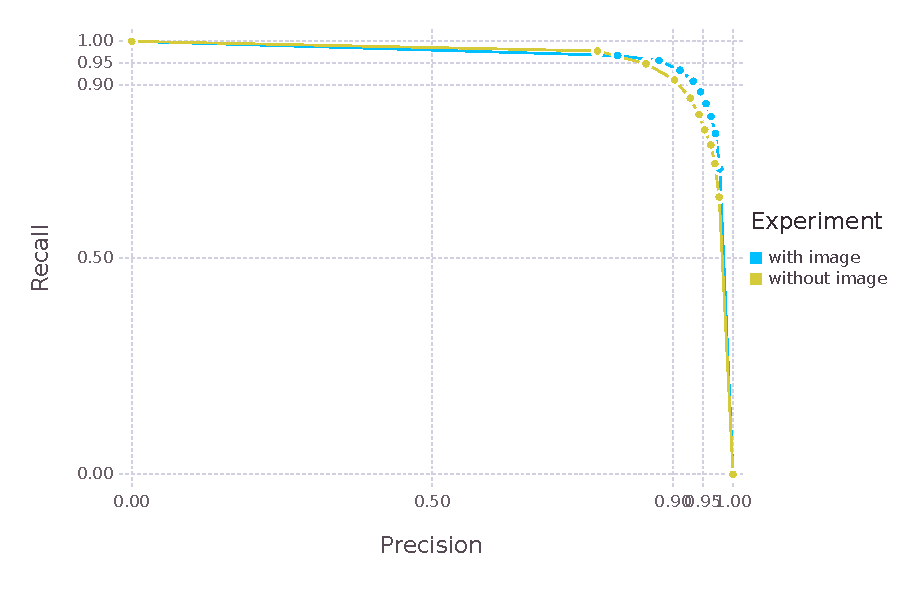
\includegraphics[width=0.65\linewidth]{pr.pdf}
	\caption{Precision and recall for error detection, both with and without access to the original image. In the test volume, there are 8266 error free locations and 961 locations with errors. In practice, we use threshold which guarantees >~95\% recall and >~85\% precision.}
	\label{fig:error_detection_pr}
\end{center}
\end{figure}

\begin{figure}
\begin{center}
	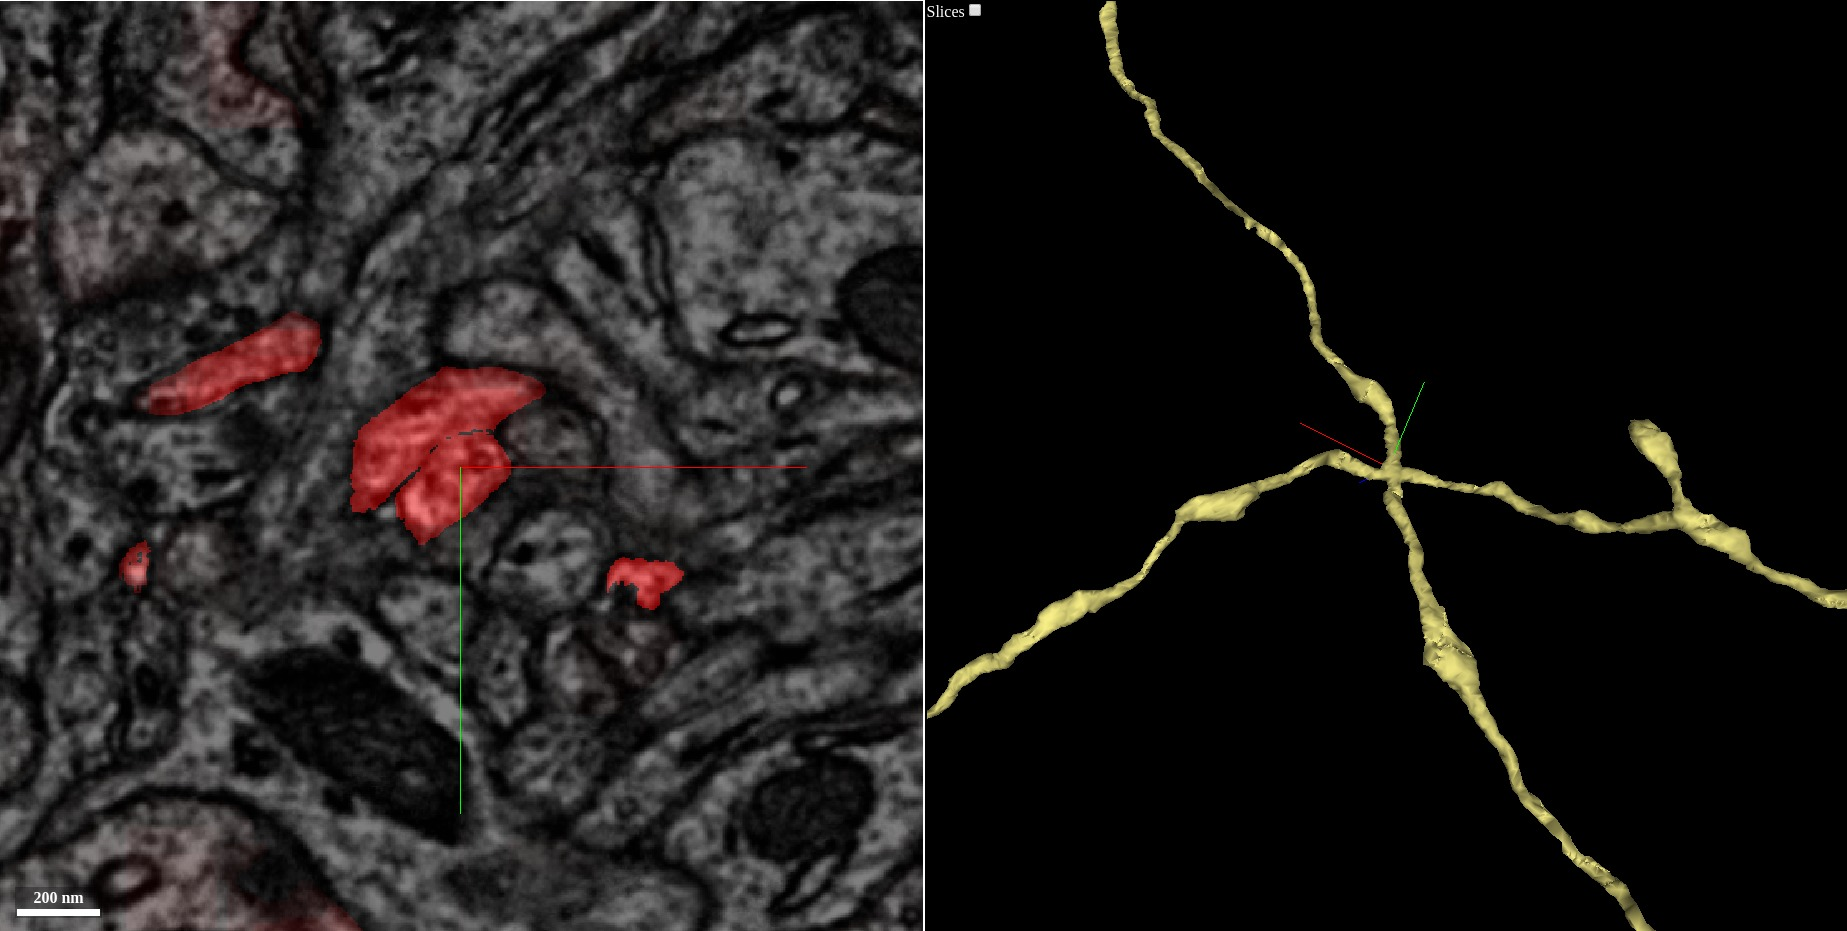
\includegraphics[width=0.65\linewidth]{x_error.jpg}
	\caption{An example of a detected error. The right shows two incorrectly merged axons, and the left shows the predicted combined error map overlaid on the corresponding 2d image in red.}
	\label{fig:x_error}
\end{center}
\end{figure}


\subsection{Error Correction Results}
\begin{figure}
\begin{center}
	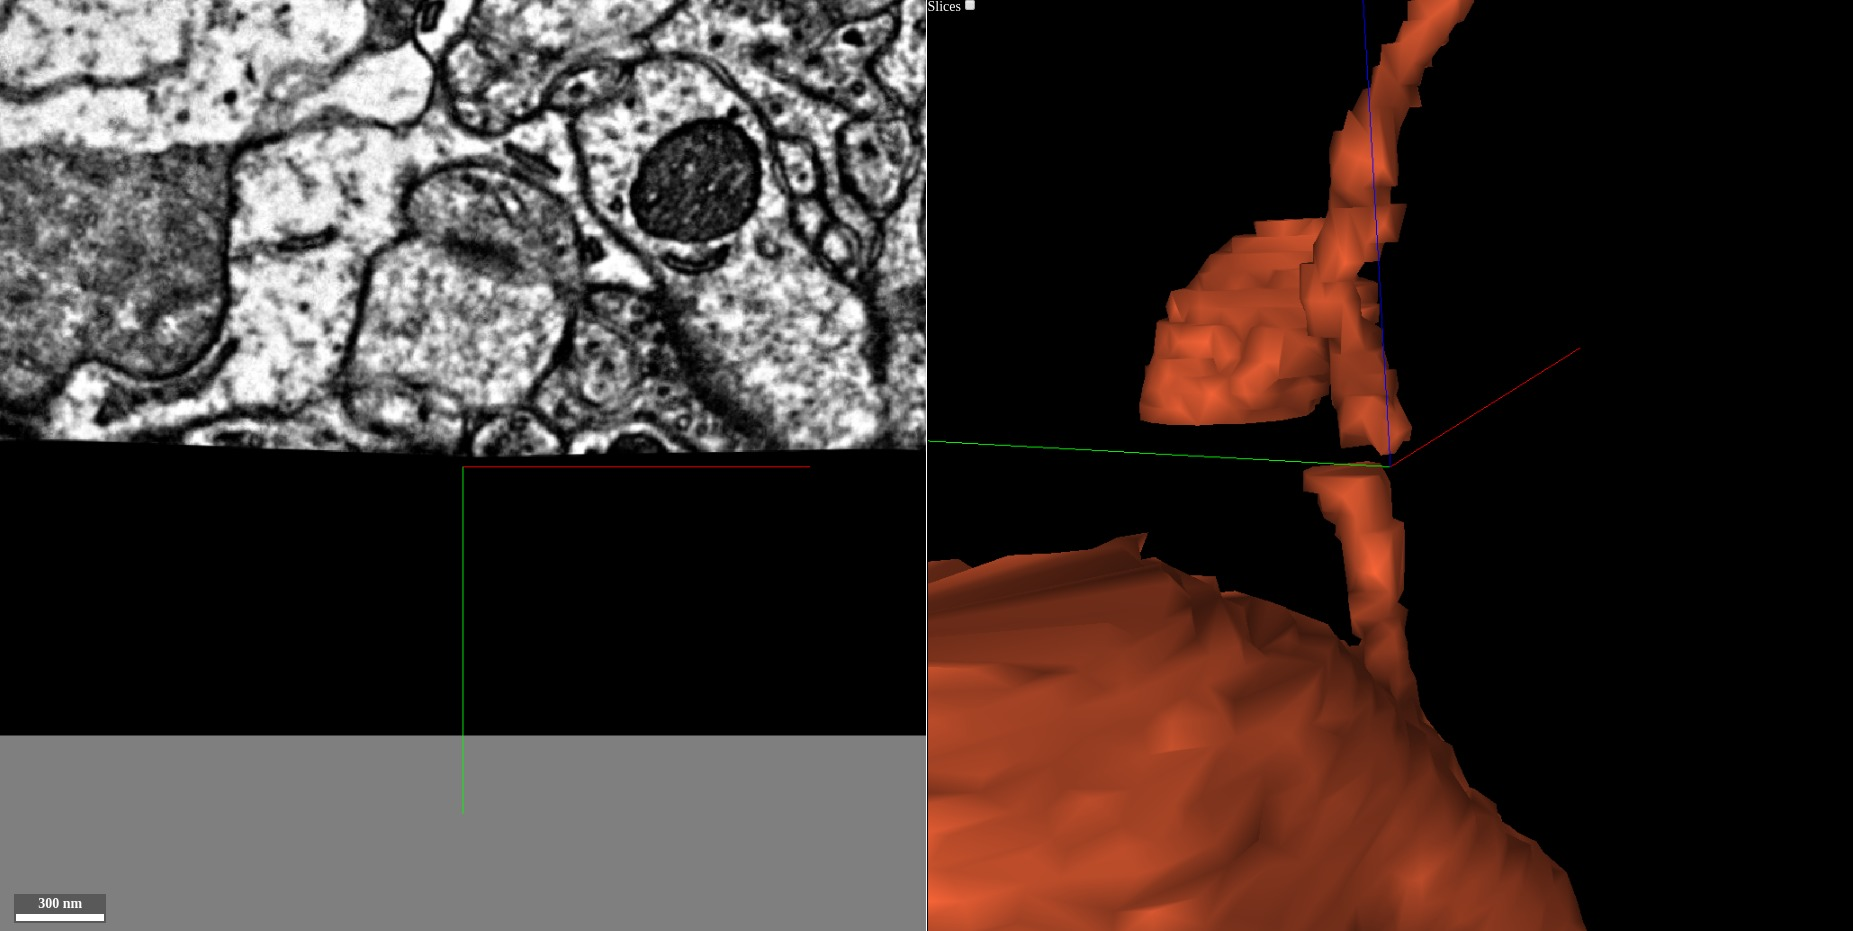
\includegraphics[width=0.65\linewidth]{difficult.jpg}
	\caption{A difficult location with missing data in one section combined with a misalignment between slices. Our algorithm was able to correctly merge across the missing data.}
	\label{fig:difficult}
\end{center}
\end{figure}
\begin{table}[h]
  \caption{Comparing segmentation performance}
  \label{table:vi_scores}
  \centering
  \begin{tabular}{lllll}
    \toprule
	& $VI_{merge}$ & $VI_{split}$ & Rand Recall & Rand Precision\\
    \midrule
    Baseline & 0.162 & 0.142 & 0.952 & 0.954\\
    Without Advice & 0.130 & 0.057 & 0.956 & 0.979\\
	With Advice & \textbf{0.088} & \textbf{0.052} & \textbf{0.974} & \textbf{0.980}\\
    \bottomrule
  \end{tabular}
\end{table}
In order to demonstrate the importance of error detection in error correction, we applied our error correction algorithm both with and without the auxiliary ``advice'' input channel having error-free objects zeroed out. The error correction network was simultaneously trained with and without advice, so this comparison is fair. Table \ref{table:vi_scores} shows that advice confers a considerable advantage in performance on the error corrector.

It is sometimes difficult to assess the significance of an improvement in variation of information or rand score since changes can be dominated by modifications to a few large objects. Therefore, we decomposed the variation of information into a score for each object in the ground truth. Recall that the variation of information between two segmentations may be computed as 
\begin{align*}
	VI_{split}&=-\frac 1 {\sum_{i,j} r_{ij}} \sum_{i,j} r_{ij} \log(r_{ij}/p_i)\\
	VI_{merge}&=-\frac 1 {\sum_{i,j} r_{ij}} \sum_{i,j} r_{ij} \log(r_{ij}/q_j)\\
	p_i&=\sum_j r_{ij}\\
	q_j&=\sum_i r_{ij}
\end{align*}
where $r_{ij}$ is the number of pixels in common between the $i^{th}$ segment of the ground truth segmentation and the $j^{th}$ segment of the proposed segmentation \cite{vi}.

We define the split and merge scores for ground truth segment $i$ as
\begin{align*}
	VI_{split}(i) &= -\sum_j r_{ij}/p_i \log(r_{ij}/p_i)\\
	VI_{merge}(i) &= -\sum_j r_{ij}/p_i \log(r_{ij}/q_j)
\end{align*}
Both quantities have units of bits. $VI_{split}(i)$ is zero iff ground truth segment $i$ is contained within a segment in the proposed segmentation, while $VI_{merge}(i)$ is zero iff ground truth segment $i$ is the union of one or more segments in the proposed segmentation. The total score $VI_{split, merge}$ is a weighted sum of the per-object scores $VI_{split,merge}(i)$. Figure \ref{fig:decomp_vi_scores} summarizes the distribution of the values of $VI(i)=VI_{merge}(i)+VI_{split}(i)$ for all segments $i$ in the ground truth.
\begin{figure}
\begin{center}
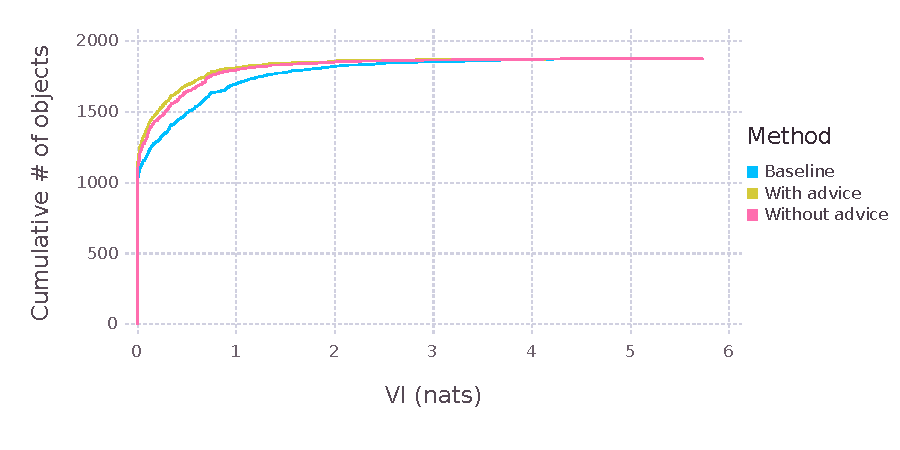
\includegraphics[width=0.65\linewidth]{per_object_vi.pdf}
\caption{Per-object vi scores for the 940 reconstructed objects in our test volume. Almost 800 objects are completely error free in our segmentation. These objects are likely all axons; almost every dendrite has a couple of errors.}
\label{fig:decomp_vi_scores}
\end{center}
\end{figure}

%Given that our baseline approach already produces state-of-the-art results on other datasets (see \cite{kisuk}), we expect that the method presented here is a substantial improvement upon the state of the art. However, we have not conducted experiments on publicly available datasets, and therefore we leave a careful comparison for future work.

\subsection{Cost Analysis}
Table \ref{table:timing} shows the cost of the most expensive parts of our segmentation pipeline. The combined cost of error detection and error correction is within an order of magnitude of the cost of boundary detection. The selectivity of our error detection network allowed us to run error correction at roughly 10\% of the possible locations in the image. Therefore, the cost of error detection is more than justified by the subsequent savings during the error correction phase. As the error rate of the initial segmentation decreases and the precision of the error detector increases, the number of locations requiring error correction will only fall further.

\begin{table}[h]
	\caption{Computation time for a volume of size $2048\times 2048\times 256$ using a single TitanX Pascal GPU}
\label{table:timing}
  \centering
  \begin{tabular}{ll}
	  \toprule
	Boundary Detection & 20 mins\\
	\midrule
	Error Detection & 25 mins\\
	\midrule
	Error Correction & 55 mins\\
	\bottomrule
  \end{tabular}
\end{table}

\section{Conclusion and Future Directions}
We have developed a segmentation error detector and demonstrated its efficacy in biasing the attention of flood filling networks. In particular, we have shown that our error detectors are able to exploit priors on neuron shape, having reasonable performance even without access to the original image. We have made significant savings in computation by applying expensive error correction procedures only where predicted necessary by the error detector. Finally, we have demonstrated that flood filling networks can benefit from the advice of error detection, improving segmentation performance upon our state-of-the-art baseline.

We expect that significant improvements in the accuracy of error detection could come from aggressive data augmentation. We can mutilate a ground truth segmentation in arbitrary (or even adversarial) ways to produce unlimited examples of errors.

An error detection module has many potential uses beyond the ones presented here. For example, we could use error detection to direct ground truth annotation effort toward mistakes. If sufficiently accurate, it could also be used directly as a learning signal for segmentation algorithms on unlabelled data.

Within the broader context of machine learning, our approach may be compared to other strategies for structured prediction problems. A relevant approach is the use of the conditional generative adversarial framework, in which one simultaneously trains a prediction network and an discriminator network which enforces structural constraints on the output \cite{cgan1,cgan2}. We do not co-train our error correction and error detection networks, but this could be the subject of future work. 

Our approach may also be compared with models for visual attention in the literature (for example, \cite{recurrent_attention}). Recurrent neural networks are able to learn in an end-to-end way how to find which parts of an image are relevant to the given task. In contrast, we have a fixed policy for which objects to attend to: we attend to those objects which likely contain errors. One of our central findings is that this policy is highly selective and improves segmentation performance.

\section{Author Contributions}
JZ conducted most of the experiments and evaluation. IT (along with
Will Silversmith) created much of the infrastructure necessary for visualization and running
our algorithms at scale. HSS secured funding and played an advisory role.

\section{Acknowledgements}
The dataset used for this project was acquired at the Allen Institute for Brain Science.
The ground truth for this project was created by Ben Silverman, Merlin Moore, Sarah Morejohn, 
Selden Koolman, Ryan Willie, Kyle Willie, and Harrison Macgowan. Kisuk Lee trained the boundary
detectors used to generate our baseline segmentation. We thank Kisuk Lee for several
helpful conversations and Nico Kemnitz for proofreading a draft of this paper. We thank 
Jeremy Maitin-Shepard and the other contributors to the neuroglancer project for creating an 
invaluable visualization tool.

We thank Barton Fiske of NVIDIA Corporation for providing us with early access to Titan X
Pascal GPU used in this research. This research was supported by the Intelligence Advanced
Research Projects Activity (IARPA) via Department of Interior/ Interior Business Center (DoI/IBC)
contract number D16PC0005. The U.S. Government is authorized to reproduce and distribute reprints
for Governmental purposes notwithstanding any copyright annotation thereon. Disclaimer: The views
and conclusions contained herein are those of the authors and should not be interpreted as necessarily
representing the official policies or endorsements, either expressed or implied, of IARPA, DoI/IBC,
or the U.S. Government.

\bibliography{bib}
\begin{appendices}
\section{Network Architectures}
\label{appendix:architecture}

\begin{figure}
\centering
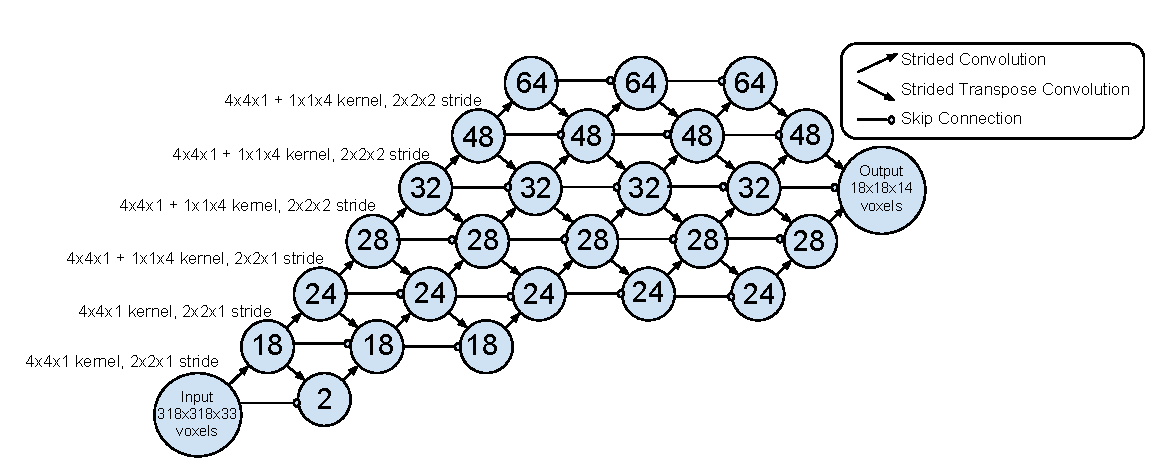
\includegraphics[width=1.0\linewidth]{error_detector.pdf}
\centering
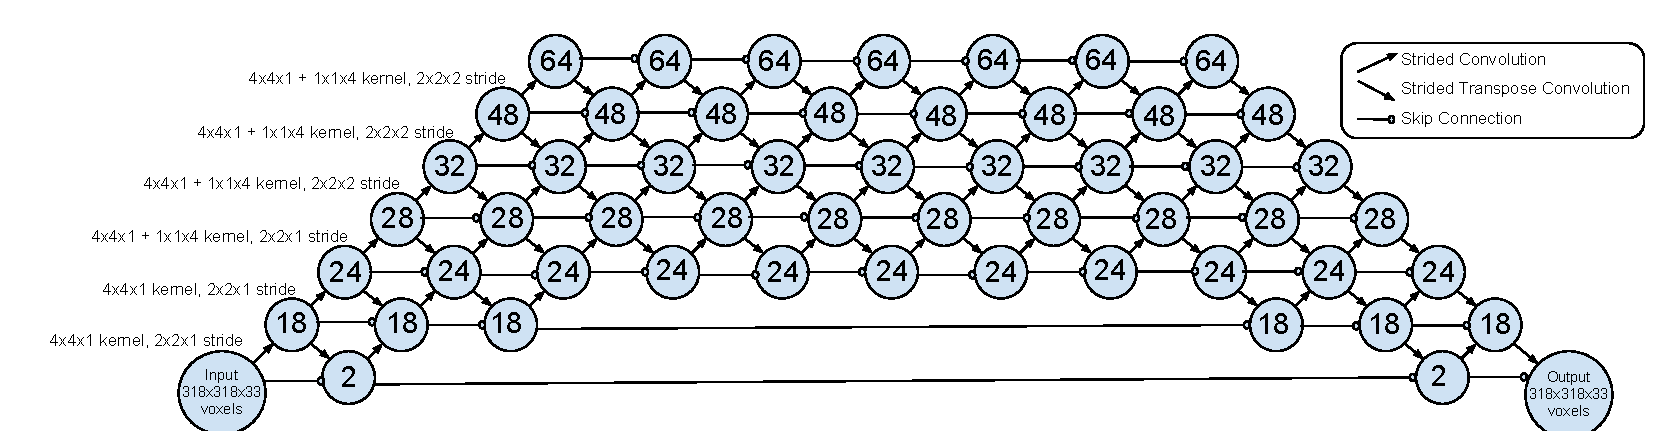
\includegraphics[width=1.0\linewidth]{error_corrector.pdf}

\caption{Architectures for the error detection and error correction modules respectively. Each node represents a layer and the number inside represents the number of feature maps. The layers closer to the top of the diagram have lower resolution than the layers near the bottom. We make savings in computation by minimizing the number of high resolution feature maps. The diagonal arrows represent strided convolutions, while the horizontal arrows represent skip connections.}
\label{fig:architecture}
\end{figure}

Due to the anisotropy of the resolution of the images in our dataset, we design our networks so that the first convolutions are exclusively 2d while later convolutions are 3D. The field of view of a unit in the higher layers is therefore roughly cubic.


To limit the number of parameters in our model, we factorize all 3D convolutions into a 2d convolution followed by a 1d convolution in z. We also use weight sharing between some convolutions at the same height.

\section{Training Details}
The neural networks were implemented in TensorFlow \cite{tensorflow} and trained using 4 TitanX Pascal GPUs with synchronous gradient descent. We used the Adam optimizer \cite{adam}.   Both networks were trained until the loss on a validation set plateaued. The error detection network trained for 700,000 iterations (approximately one week), while the error correction network trained for 1,700,000 iterations (approximately three weeks).
\end{appendices}


\end{document}
